\documentclass[11pt]{article}
\usepackage{graphicx}
\usepackage{amsmath}
\usepackage{geometry}
\usepackage{indentfirst}
\usepackage{mathbbol}
\usepackage{float}
\usepackage{listings}
\usepackage{xcolor}
\usepackage{hyperref}

\definecolor{mygray}{gray}{0.9}

\geometry{
a4paper,
left=25mm,
top=30mm,
bottom=30mm,
right=20mm}

\lstset{
   showstringspaces=false
}

\title{Independent Study : Implementation of Non-linear Workbook in Python}
\author{Prajwal Padmanabha under supervision of Dr. Ananda Dasgupta}
\date{}

\begin{document}

	\maketitle
	\section*{Introduction}
		The book `The Nonlinear Workbook' by Willi Hans Steeb is a toolbox of various algorithms and methods used in the field of non-linear dynamics. The book contains the tools and brief overview of the math behind the tools, ranging from chaos to genetic algorithms to neural networks. In addition to this, the book also lists implementation of the algorithm in C++ and Java. This book is of immense use for anyone foraying into the field of scientific computation. 

		One of the widely used languages in computation in science is Python. The main reasons behind this are the ease of coding and the availability of numerous packages for specific purposes. The goal of the independent study is to study the algorithms and tools listed in the book and to recreate them in Python (using plain python and at places possible, the available additional packages). 
	
	\section{Nonlinear and Chaotic Maps}
		A map is a function $f : S \rightarrow S$ where $S \subset \mathbb{R}$. \\

		For continuous time, a differential equation would be $\dot{x} = f(x)$ while a discrete time evolution would be written as $x_{t+1} = f(x_t)$ and this is called a difference equation. In both cases, $x_0 \in S$.\\

		The sequence $ x_0, f(x_0), f(f(x_0)) ....$ is called the trajectory of $x_0$. In this trajectory, a point is a fixed point of the map if $x^{*} = f(x^{*})$ and periodic if $x^* = f^{(n)}(x^*)$. We consider some examples of maps and check for periodicity and fixed points in them.

		\subsection{Trajectories and Periodicity in One Dimension}

			\textbf{Example 1 : A Simple map}
			$$
			f(x) = 
			\begin{cases} 
				\frac{x}{2} & $x is even$\\
				3 x + 1 & $x is odd$
   			\end{cases}
   			$$

   			From Figure 1, it can be seen that  the map goes below $y=x$ if x is even and goes above $y=x$ and lands on an even point otherwise.

   			\begin{figure}[H]
	   			\centering	
   				\includegraphics[width=4in]{fig/{1.1.1}.png}
   				\caption{Example 1}
   			\end{figure}

			\textbf{Example 2 : Logistic Map}
			$$
			f(x) = r x (1-x)
   			$$

            The parameter r=4 in the example given below. The logistic map is an excellent map to study chaotic behaviour as it proceeds from stable to periodic to chaotic depending on the value of r (see Figure 3).

   			\begin{figure}[H]
	   			\centering	
   				\includegraphics[width=4in]{fig/{1.1.2}.png}
   				\caption{Example 2}
   			\end{figure}

            \begin{figure}[H]
               \centering  
               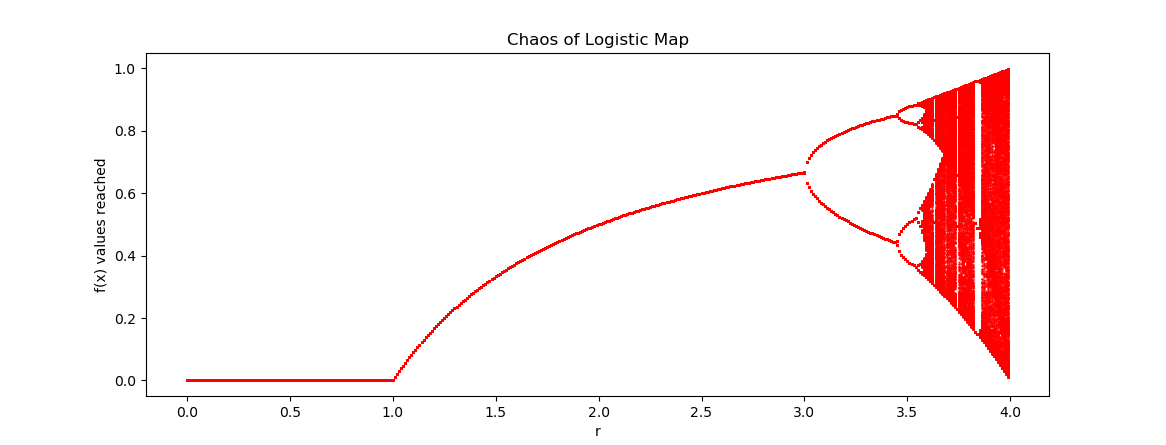
\includegraphics[width=7in]{fig/logisticBif.png}
               \caption{Logistic Map Bifurcation. r: Growth Rate}
            \end{figure}

			\textbf{Example 3 : Bernoulli Map}
			$$
			f(x) = 
			\begin{cases} 
				2 x & x \leq 0.5\\
				2 x - 1 & $ otherwise$
   			\end{cases}
   			$$

   			\begin{figure}[H]
	   			\centering	
   				\includegraphics[width=4in]{fig/{1.1.3}.png}
   				\caption{Example 3 : Bernoilli Map}
   			\end{figure}

			\textbf{Example 4 : Bungalow Tent Map}
			$$
			f_a(x) = 
			\begin{cases} 
				\dfrac{1-a}{a} x & x \in [0,a) \\ \\
				\dfrac{2a}{1-2a}x + \dfrac{1-3a}{1-2a} & x \in [a,0.5) \\ \\
				\dfrac{2a}{1-2a}(1-x) + \dfrac{1-3a}{1-2a} & x \in [0.5,1-a) \\ \\
				\dfrac{1-a}{a}(1-x) & x \in [1-a,1]
   			\end{cases}
   			$$

            The value of a used is 1/3. Depending on the value of a, various properties can be found (such as stable points, periodic points). See code for implementation.

   			\begin{figure}[H]
	   			\centering	
   				\includegraphics[width=4in]{fig/{1.1.4}.png}
   				\caption{Example 4 : Bungalow Tent Map}
   			\end{figure}

			\textbf{Example 5 : Gauss Map}
			$$
			f(x) = 
			\begin{cases} 
				0 & x = 0\\
				[1/x] & $otherwise$
   			\end{cases}
   			$$

   			where $[n]$ denotes fractional part of n .\\

   			\begin{figure}[H]
	   			\centering	
   				\includegraphics[width=4in]{fig/{1.1.5}.png}
   				\caption{Example 5 : Gauss Map}
   			\end{figure}



   			The codes to print the trajectories of these maps can be found in \textbf{Appendix A}.\\ \\
   			Certain points to be noted with regard to code:

   			1. Unlike C++ or Java, no new \textit{long int} variable needs to be declared in Python to handle large values since there is no upper bound on the value of memory assigned to a variable. The disadvantage of this is, if a large number is given, the program will not terminate with an overflow error and instead will continue drawing more memory.

   			2. For maps like Bernoulli Map and Tent Map, taking floating point numbers may not be accurate representation of fractional values since these maps are chaotic and sensitive to initial conditions. Taking this into account, the code has been written with a provision to do computation in fractional mode. The caveat here is that the numerator and denominator can quickly become large values (in Bernoulli map), which slows down computation significantly.

   		\subsection{Invariant Density}
   			Consider a fully chaotic, one hump map, $f(x)$. Then, invariant density can be defined as 
   			$$\rho(x) = \lim_{T\to\infty}\frac{1}{T}\sum_{t=0}^{T-1} \delta\big(x-f^{(t)}(x_0)\big)$$

   			This function acts as a measure of how many times a point has been visited, i.e, like a probability density. We shall see that this is equivalent to a probability density. Due to this, there is a need for the function to be fully chaotic. If the function is not fully chaotic, i.e, there exists an attractor, or a periodicity, the function ends up at a finite set of points making the invariant density exist only at those points. Using the logistic map, we shall see examples of this.

   			The reason for function to be one hump is not clearly understood. An example of double hump map also shows invariant density. Further investigation needs to be done in this matter. \\ \\
   			\textbf{Some properties of Invariant Density}\\

   			Consider an integrable function $g(x)$. Then,
   			$$
   				\langle g(x) \rangle = \lim_{T\to\infty} \frac{1}{T} \sum_{t=0}^{T-1} g(x_t) = \int_0^1\rho(x)g(x)dx
   			$$

   			Setting $g(x) = 1$, we obtain, just like a probability density,
   			$$
   				\int_0^1\rho(x)dx = 1
   			$$

   			Let us define 
   			$$
   				\sigma (y) := \int_0^1\delta\big(y - f^k(x)\big) \rho(x)dx
   			$$
   			Then,
   			\begin{align*}
   				\int_0^1 \sigma(y) g(y) dy &= \int_0^1 \int_0^1 \delta \big(y - f^k(x)\big)\rho(x)g(x)dxdy = \int_0^1 \rho(x)g(x_k)dx \\ 
   				&= \lim_{T\to\infty} \frac{1}{T} \sum_{t=0}^{T-1} \int_0^1 \delta \big( x-f^t(x_0) \big) g(f^k(x_0))dx\\
   				& = \lim_{T\to\infty} \frac{1}{T} \sum_{t=0}^{T-1} g\big(f^{t+k}(x_0)) = \lim_{T\to\infty} \frac{1}{T} \sum_{t=0}^{T-1} \int_0^1 \delta \big(y-f^{t+k}(x_0)\big)g(y)dy \\
   				& = \int_0^1 \rho(y) g(y) dy
   			\end{align*}
   			Since $\sigma$ was arbitrary, we can state $\sigma(y) = \rho (y)$. Hence, setting $k=1$ in definition of $\sigma$, we get
   			\begin{align*}
   				&\rho (y) = \int_0^1 \rho(x) \delta \big(y-f(x)\big)dx \\
   				& \implies \rho_{t+1}(y) = \int_0^1 \rho_t(x) \delta \big(y-f(x)\big)dx 
   			\end{align*}
   			And this allows us to find out the invariant density as $T\to\infty$ by time evolution of $\rho_0(x)$\\ \\
            \newpage
   			\textbf{Examples of Invariant Densities}\\

            The invariant densitites were calculated for different starting points. From the figures, it is seen that the invariant density is, for the lack of a better term, invariant. \\
            
            \textbf{Example 1 : Bungalow Tent Map}
               \begin{figure}[H]
               \centering  
               \includegraphics[width=5.5in]{fig/{1.1.3BungTent}.png}
               \caption{Invariant Density for Bungalow Tent Map}
            \end{figure}

            \textbf{Example 2 : Double Hump Map}

            This example is to check what happens when a Double Hump Map is used. The map used was 

            $$
               f(x) = 
               \begin{cases} 
                  r(\frac{1}{2}-x)x & x<\frac{1}{2}\\
                  r(1-x)(x-\frac{1}{2}) & $otherwise$
                  \end{cases}
            $$

            The double hump map looks like this:
             \begin{figure}[H]
               \centering  
               \includegraphics[width=3.5in]{fig/{doubleHumpMap}.png}
               \caption{Double Hump Map}
            \end{figure}

            with the bifurcation diagram looking like:
             \begin{figure}[H]
               \centering  
               \includegraphics[width=4.5in]{fig/{doubleHumpChaos}.png}
               \caption{Bifurcation Diagram for Double Hump Map}
            \end{figure}

            This confirms the chaotic behaviour of double hump map at appropriate values of r. The invariant density for this map looks such:

             \begin{figure}[H]
               \centering  
               \includegraphics[width=5.5in]{fig/{1.1.3DoubHump}.png}
               \caption{Invariant Density for Double Hump Map}
            \end{figure} 

            \textbf{Example 3 : Logistic Map}

             \begin{figure}[H]
               \centering  
               \includegraphics[width=5.1in]{fig/{1.1.3Logistic}.png}
               \caption{Invariant Density for Logistic Map}
            \end{figure}


            \textbf{Example 4 : Sine Map}
             \begin{figure}[H]
               \centering  
               \includegraphics[width=4.5in]{fig/{1.1.3Sine}.png}
               \caption{Invariant Density for Sine Map}
            \end{figure}

            \textbf{Time Evolution}\\

               Using the time evolution formula derived earlier, starting from $\rho(x)=1$, invariant density time evolution was tried for logistic map, resulting in this:
            \begin{figure}[H]
               \centering  
               \includegraphics[width=4.5in]{fig/{1.1.3TimeEvol}.png}
               \caption{Time Evolution of Invariant Density for Logistic Map}
            \end{figure}
            The generated figure is quite close to the invariant density calculated and plotted previously, verifying the method of time evolution.


   		\subsection{Discrete Fourier Transform}
   			Let $f(t)$ be a continuous time signal, sampled at $N$ points, $f[0],f[1],...,f[N-1]$. Fourier transform of $f(t)$ is given by (barring normalization)
   			$$
   				F(\omega)=\int_{-\infty}^\infty f(t) e^{-i \omega t} dt
   			$$
   			The samples points $f[n]$ is equivalent to an impulse in $\Delta t$ having area $f[n]$. Then,
   			\begin{align*}
   				F[\omega] &= \int_0^{T (N-1)} f(t) e^{- i \omega t}dt  \\
   				&= f[0] e^{-i \omega \times 0} + f[1] e^{-i \omega \times 1} +...+ f[N-1] e^{-i \omega \times T(N-1)} \\
   				&= \sum_{n=0}^{N-1} f[n] e^{- i \omega n T}
   			\end{align*}
   			Analogous to the fundamental time period after which the signal repeats in Fourier expansion, since the sampling is done only from 0 to N-1, we can assume that the signal repeats after the N-1 time sampling. Hence, we can write
   			$$
   				\omega = 0, \frac{2\pi}{N T},2 \times \frac{2\pi}{N T},...,(N-1) \times \frac{2\pi}{N T}
   			$$
   			This gives us the expression for discrete fourier transform:
   			$$
   				F[k] = \sum_{n=0}^{N-1} f[n] e^{-i\frac{ 2\pi n k }{N}}
   			$$
   			and with normalization, 
   			$$
   				F[k] = \frac{1}{N}\sum_{n=0}^{N-1} f[n] e^{-i\frac{ 2\pi n k }{N}}
   			$$
   			This can be rewritten as a matrix equation:
   			$$
   				\vec F = D \vec f
   			$$
   			$$
   				[D]_{ij} = \frac{1}{N} W^{ij} \qquad \textrm{where} \; W = e^{-i\frac{2\pi}{N}}
   			$$
   			Since this is a matrix multiplication with a vector, the order complexity of this operation is $\mathcal{O} (n^2)$ \\[10mm]
            \textbf{DFT of cosine map}

            The map considered is $x(t) = cos\Big(\dfrac{2 \pi t}{N}\Big)$ sampled at $t=0,1,...,N-1$. The DFT for this is given analytically by 
            $$
               X[k] = 
               \begin{cases} 
                  \frac{1}{2} & k = 1\\
                  \frac{1}{2} & k = N-1\\
                  0 &\textrm{otherwise}
                  \end{cases}
            $$

            \begin{figure}[H]
               \centering  
               \includegraphics[width=4.5in]{fig/{1.1.6Cosine}.png}
               \caption{DFT for Cosine Map}
            \end{figure}

            \textbf{DFT of Logistic Map}\\

            DFT of a logistic map shows interesting properties. We assume that we have N samples from the logistic map. Depending on the value of $r$ we see different results. $r=4$ shows chaos in the DFT. $r=3.2$ shows two period and $r=3.5$ shows four period which is consistent with the bifurcation diagram of logistic map. 

            \begin{figure}[H]
               \centering  
               \includegraphics[width=4.6in]{fig/{1.1.6Logr-2.9}.png}
               \caption{DFT for Logistic Map with r=2.9}
            \end{figure}

            \begin{figure}[H]
               \centering  
               \includegraphics[width=4.7in]{fig/{1.1.6Logr-3.2}.png}
               \caption{DFT for Logistic Map with r=3.2}
            \end{figure}

            \begin{figure}[H]
               \centering  
               \includegraphics[width=4.8in]{fig/{1.1.6Logr-3.5}.png}
               \caption{DFT for Logistic Map with r=3.5}
            \end{figure}

            \begin{figure}[H]
               \centering  
               \includegraphics[width=4.8in]{fig/{1.1.6Logr-4}.png}
               \caption{DFT for Logistic Map with r=4}
            \end{figure}

          \textbf{Time Complexity of DFT}\\

          From the derivation, it is seen that DFT can be written as a matrix multiplication. The following figure shows the time complexity for various values of N, verifying the complexity.

           \begin{figure}[H]
               \centering  
               \includegraphics[width=4.8in]{fig/{1.1.6TimeComp}.png}
               \caption{Time Comparison for DFT with Cosine Map}
            \end{figure}

         \subsection{Fast Fourier Transform}
            The DFT explained in the previous subsection is of the order of $\mathcal{O}(n^2)$ which can become very slow of large values for n (as is obtained in time series data). To make this more efficient, some properties in the DFT must be noted.

            Ignoring normalization constant, the DFT is given by 
            $$
               F[k] = \sum_{n=0}^{N-1} f[n] e^{-i\frac{ 2\pi n k }{N}} = \sum_{n=0}^{N-1} f[n] \; W_N^{nk}
            $$
            Certain values of $W_N^{nk}$ repeat multiple times due to:

            1. The value of product $nk$ repeats multiple times.

            2. $W_N^{nk}$ represent the roots of unity. These have repeated absolute values (assuming N is even). \\[5mm]
            To give an example, $N=8$. Then,
            \begin{align*}
              & W_8^1 = e^{-i\frac{2\pi}{8}} = \frac{1 - i}{\sqrt{2}} \; := a \\
               &W_8^2 = a^2 = -i \\
               &W_8^3 = a^3 = -i a = a^* \\
               &W_8^4 = a^4 = -1 \\
               &W_8^5 = a^5 = -a \\
               &W_8^6 = a^6 = i \\
               &W_8^7 = a^7 = i a = -a^* \\
               &W_8^8 = a^8 = 1
            \end{align*}
            Since any $nk$ falling outside 0 to 7 can be written as a modulo 8 value falling within 0 to 7. Hence, only four values are needed, $a, a^*, i, 1$, which simplifies the computation speeding up DFT. This is the core idea used in Fast Fourier Transform. 
            
            One algorithm for performing FFT is called Decimation in Time algorithm. This splits the summation over k into two parts. (Note: let us assume that $N=2^p$ for some value p)
            \begin{align*}
               &m = \frac{k}{2} \; \textrm{if k is even} \\
               &m = \frac{k-1}{2} \; \textrm{if k is odd}
            \end{align*}
            Then,
            \begin{align*}
               &F[k] = \sum_{m=0}^{\frac{N}{2} - 1} f[2m]\; W_N^{2mk} + \sum_{m=0}^{\frac{N}{2} - 1} f[2m+1]\; W_N^{(2m+1)k}\\
               &\textrm{Note that} \; W_N^{2mk} =  e^{-i\frac{2\pi}{N} 2mn} = e^{-i\frac{2\pi}{N/2} mn} = W_{\frac{N}{2}}^{mn}\\
               &\implies F[k] = \sum_{m=0}^{\frac{N}{2} - 1} f[2m]\; W_{N/2}^{mk} + \sum_{m=0}^{\frac{N}{2} - 1} f[2m+1]\; W_{N/2}^{mk}\; W_{N}^{k}\\
               &\implies F[k] = G[k] + W_N^k \; H[k]
            \end{align*}
            which is a two $\frac{N}{2}$ order DFT. This process can be iterated until two point DFT is reached (hence the assumption of N as a power of 2).

         \subsection{Lyapunov Exponent}
            Lyaponov exponent characterizes how infinitesimally close trajectories change with time. \\ \\
            Let $x^*(t)$ and $x(t)$ be two trajectories of the map $x_{t+1} = f(x_t)$ with $x^*(0)$ and $x(0)$ being infinitesimally close. Then,
            \begin{align*}
            &y_t := x^*_t - x_t\\
            &\implies y_{t+1} = x^*_{t+1} - x_{t+1} = f(x^*_t) - f(x_t)\\
            &\textrm{Doing Taylor expansion around $x_t$, we get} \; y_{t+1} = (x^*_t - x_t) \frac{df(x_t)}{dx} = y_t  \frac{df(x_t)}{dx}
            \end{align*}
            In a continuous system, this would give the solution $y(t) = y(0) e^{\lambda t}$. $\lambda$ is called the Lyapunov exponent. In a n dimensional system, there is a spectrum of Lyapnunov exponents $\lambda_1, \lambda_2 ... \lambda_n$. Maximal Lyapunov exponent is defined as 
            $$
            \lambda = \lim_{t \to \infty} \lim_{y_0 \to 0} \frac{1}{t} log\frac{|y(t)|}{|y_0|}
            $$
            In a discrete time system, this translates to
            \begin{align*}
               &\lambda(x_0,y_0) := \lim_{T\to\infty} \frac{1}{T} log |\frac{y_T}{y_0}|\\
               & \textrm{Since} \; f^{'}(x_t) = \frac{y_{t+1}}{y_t}, \\
               &\lambda(x_0,y_0) = \lim_{T\to\infty} \sum_{t=0}^{T} \frac{1}{T} log(|f^{'}(x_t)|)
            \end{align*}
            If $\lambda > 0$ , this means that infinitesimally close trajectories exponentially grow apart in time. This is a measure of chaos of the system in the sense that it is very sensitive to initial conditions and any small perturbation will lead to a butterfly effect over time. \\
            Note that $\lambda$ depends on the inital point $x_0$. Hence, if $x_0$ is a fixed point or a periodic point or eventually periodic, the Lyapunov exponent will be the sum of constant terms. If the slope at that point is less than 1, then $\lambda$ is negative (0 if slope is less than $e$ and diverges otherwise). Hence, calculating Lyaponov exponents for those points is pointless. \\[5mm]   \newpage       
            \textbf{Lyapunov exponent for Logistic map with r=4}

            \begin{figure}[H]
               \centering  
               \includegraphics[width=5.5in]{fig/{1.1.4lyap}.png}
               \caption{Lyapunov Exponents for Logistic Map}
            \end{figure}

            Fromt he figure, apart from 0.5 having a low value (since it is a point that leads to 0), most of the points have 0.69 (= $log(2)$). In practice, however, this is only considering a sufficiently well placed set of points. There are countably infinite points that are eventually periodic or eventually lead to 0 which is a fixed points. For points like these, the lyapunov exponents will be 0 and this can be observed by increasing the total time considered and decreasing the spacing between the points. For purposes of clarity, this has been avoided to show that most points (the uncountably infinite points between the points mentioned above) have a positive Lyapunov exponent indicating chaos.

         \subsection{Autocorrelation Function}
            Let $x_{t+1} = f(x_t)$. Then, the time average of x is, $\langle x \rangle = \lim_{T\to\infty}\frac{1}{T}\sum_{t=0}^{T-1}x_t$. Autocorrelation function can then be defined as:
            $$
               C_{xx}(\tau) = \lim_{T\to\infty}\frac{1}{T} \sum_{t=0}^{T-1}(x_t - \langle x\rangle)(x_{t+\tau} - \langle x\rangle)
            $$
            Autocorrelation function is a measure of the correlation in time series data. Hence, it can be used as a check for randomness in the system (i.e, $C_{xx}(\tau) \to 0$ as $\tau \to \infty$). In the event of correlation existing i.e, non randomness, it can give clues about the underlying model of the time series data.\\[5mm] \newpage
            \textbf{Autocorrelation Function for Logistic Map}

            \begin{figure}[H]
               \centering  
               \includegraphics[width=5.5in]{fig/{1.1.5autoCor}.png}
               \caption{Autocorrelation Map for different starting points in Logistic Map}
            \end{figure}
      \newpage
      \section*{Appendix A : Codes}

      All the codes have been written using Python3. Some of the codes may require additional packages such as NumPy and Matplotlib for plotting and efficient array computation purposes. All the codes can be found at \url{https://github.com/prajwalp/nlwPy}\\

      \subsection*{A1 : Trajectories in 1D}
      \textbf{1.1.1ex1.py}
      \begin{lstlisting}[backgroundcolor = \color{mygray},breaklines=true,language=Python]
#1.1.1 Example 1 :Trajectory of defined map

def f(n0):
   if(int(str(int(n0))[-1])%2 == 0): #Using string formatting to check if number is even
      n0 = n0/2
   else:
      n0 = 3*n0 + 1
   return n0

n0 = int(input('Enter the starting number: '))
t = int(input('Enter the number of iterations: '))

#Defining list for storing time evolution
l=[]
l.append(n0)

#Check for periodicity
e=0

#Time evolution loop
for i in range(t):
   n0=f(n0)
   if(e==0 and n0 in l):
      e = 1
   l.append(n0)
   print(n0)
if (e==1):
   print('The starting point is eventually periodic')
      \end{lstlisting}
      \vspace{10mm}
      \textbf{1.1.1ex2.py}
      \begin{lstlisting}[backgroundcolor = \color{mygray},breaklines=true,language=Python]
#1.1.1 Example 2: Logistic Map trajectory

import fractions as fr
import math

#Logistic Map
def f(x):
   return 4*x*(1-x)

check = int(input('Enter 1 for fractional mode or 2 for float mode: '))

if(check == 1):
   #Allowing for fractional input since number is between 0 and 1
   num = int(input('Enter numerator of starting point: '))
   den = int(input('Enter denominator of starting point: '))
   y0 = fr.Fraction(num,den)
   y=y0
else:
   y0 = float(input('Enter the starting point: '))
   y=float(y0)

t = int(input('Enter the number of iterations: '))

for i in range(t):
   y = f(y)
   print(float(y))

#Error between analytical and numerical value
x_true = 0.5 - 0.5 * math.cos(2**t * math.acos(1-2*y0))
err = x_true - y

print('Error between exact and numerical value: ',err)


      \end{lstlisting}
      \vspace{10mm}
      \textbf{1.1.1ex3.py}
      \begin{lstlisting}[backgroundcolor = \color{mygray},breaklines=true,language=Python]
#Example 3: Bernoulli map trajectory

import fractions as fr
import math

def f(x):
   if(x<0.5):
      return 2*x
   else:
      return 2*x - 1

check = int(input('Enter 1 for fractional mode or 2 for float mode: '))

if(check == 1):
   num = int(input('Enter numerator of starting point: '))
   den = int(input('Enter denominator of starting point: '))
   y0 = fr.Fraction(num,den)
   y=y0
else:
   y0 = float(input('Enter the starting point: '))
   y=float(y0)

t = int(input('Enter the number of iterations: '))

l=[]
l.append(y)
e=0

for i in range(t):
   y = f(y)
   if(e==0 and y in l):
      e = 1
   l.append(y)
   print(float(y))

if (e==1):
   print('The starting point is eventually periodic')


      \end{lstlisting}
      \vspace{10mm}
      \textbf{1.1.1ex4.py}
      \begin{lstlisting}[backgroundcolor = \color{mygray},breaklines=true,language=Python]
#Example 4: Bungalow Tent map trajectory

import fractions as fr
import math


def f(x,a):
   if(x<a):
      return (1-a)*x/a
   elif(x<0.5):
      return 2*a*x/(1-2*a) + (1-3*a)/(1-2*a)
   elif(x<1-a):
      return 2*a*(1-x)/(1-2*a) + (1-3*a)/(1-2*a)
   else:
      return (1-a)*(1-x)/a


check = int(input('Enter 1 for fractional mode or 2 for float mode: '))

if(check == 1):
   num = int(input('Enter numerator of starting point: '))
   den = int(input('Enter denominator of starting point: '))   
   y0 = fr.Fraction(num,den)
   y=y0
   num = int(input('Enter numerator of control parameter: '))
   den = int(input('Enter denominator of control parameter: '))   
   a0 = fr.Fraction(num,den)
   a=a0

else:
   y0 = float(input('Enter the starting point: '))
   a= float(input("Enter the control parameter: "))   
   y=float(y0)

t = int(input('Enter the number of iterations: '))

l=[]
l.append(y)
e=0

for i in range(t):
   y = f(y,a)
   if(e==0 and y in l):
      e = 1
   l.append(y)
   print(float(y))

if (e==1):
   print('The starting point is eventually periodic')



      \end{lstlisting}
      \vspace{10mm}
      \textbf{1.1.1ex5.py}
      \begin{lstlisting}[backgroundcolor = \color{mygray},breaklines=true,language=Python]
#Example 5: Gauss map trajectory

import fractions as fr
import math

def f(x):
   if(x==0):
      return 0
   else:
      return 1/x-math.floor(1/x)

check = int(input('Enter 1 for fractional mode or 2 for float mode: '))

if(check == 1):
   num = int(input('Enter numerator of starting point: '))
   den = int(input('Enter denominator of starting point: '))
   y0 = fr.Fraction(num,den)
   y=y0
else:
   y0 = float(input('Enter the starting point: '))
   y=float(y0)

t = int(input('Enter the number of iterations: '))

l=[]
l.append(y)
e=0

for i in range(t):
   y = f(y)
   if(e==0 and y in l):
      e = 1
   l.append(y)
   print(float(y))

if (e==1):
   print('The starting point is eventually periodic/leads to a fixed point')


      \end{lstlisting}
      \subsection*{A2 : Invariant Density}
      \textbf{1.1.3invDenBungTent.py}
      \begin{lstlisting}[backgroundcolor = \color{mygray},breaklines=true,language=Python]
#Invariant Density for Bungalow Tent Map

import matplotlib.pyplot as plt

#Bungalow Tent Map
def f(x,a):
   if(x<a):
      return (1-a)*x/a
   elif(x<0.5):
      return 2*a*x/(1-2*a) + (1-3*a)/(1-2*a)
   elif(x<1-a):
      return 2*a*(1-x)/(1-2*a) + (1-3*a)/(1-2*a)
   else:
      return (1-a)*(1-x)/a

#invariant density function
def rhoFun(x0,T):
   rho=[]
   xi=x0
   for i in range(T):
      rho.append(f(xi,0.25))
      xi=f(xi,0.25)
   return rho


fig,ax=plt.subplots(2,2)
plt.subplots_adjust(wspace=0.4,hspace=0.5)
x0Val=[[0.2,0.4],[0.6,0.8]]

#loop over axes in subplot, plotting histogram of time evolution
for xAx in range(2):
   for yAx in range(2):
      x0=x0Val[xAx][yAx]
      rho=rhoFun(x0,10000)
      axCur=ax[xAx][yAx]
      axCur.hist(rho,bins=25,density='True')
      axCur.set_title('x0: %.2f'%x0)
      axCur.set_xlabel('x')
      axCur.set_ylabel('Density of x')
fig.suptitle('Bungalow Tent Map invariant Density | a: %.2f'%0.25)
plt.show()
      \end{lstlisting}
      \vspace{10mm}
      \textbf{1.1.3invDenDoubleHump.py}
      \begin{lstlisting}[backgroundcolor = \color{mygray},breaklines=true,language=Python]
#Invariant Density for Double Hump Map

import matplotlib.pyplot as plt
import math

#Double hump
def f(x):
   if(x<0.5):
      return 16*(0.5-x)*x
   else:
      return 16*(1-x)*(-0.5+x)

#invariant density function
def rhoFun(x0,T):
   rho=[]
   xi=x0
   for i in range(T):
      rho.append(f(xi))
      xi=f(xi)
   return rho


fig,ax=plt.subplots(2,2)
plt.subplots_adjust(wspace=0.4,hspace=0.5)
x0Val=[[0.2,0.4],[0.6,0.8]]

#loop over axes in subplot, plotting histogram of time evolution
for xAx in range(2):
   for yAx in range(2):
      x0=x0Val[xAx][yAx]
      rho=rhoFun(x0,10000)
      axCur=ax[xAx][yAx]
      axCur.hist(rho,bins=25,density='True')
      axCur.set_title('x0: %.2f'%x0)
      axCur.set_xlabel('x')
      axCur.set_ylabel('Density of x')
fig.suptitle('Double Hump Map invariant Density | r=16')
plt.show()
      \end{lstlisting}
      \vspace{10mm}
      \textbf{1.1.3invDenLogistic.py}
      \begin{lstlisting}[backgroundcolor = \color{mygray},breaklines=true,language=Python]
#Invariant Density for Logistic Map

import matplotlib.pyplot as plt

#Logistic Map with r=4
def f(y):
   return 4*y*(1-y)

#invariant density function
def rhoFun(x0,T):
   rho=[]
   xi=x0
   for i in range(T):
      rho.append(f(xi))
      xi=f(xi)
   return rho


fig,ax=plt.subplots(2,2)
plt.subplots_adjust(wspace=0.4,hspace=0.5)
x0Val=[[0.2,0.4],[0.6,0.8]]

#loop over axes in subplot, plotting histogram of time evolution
for xAx in range(2):
   for yAx in range(2):
      x0=x0Val[xAx][yAx]
      rho=rhoFun(x0,10000)
      axCur=ax[xAx][yAx]
      axCur.hist(rho,bins=25,density='True')
      axCur.set_title('x0: %.2f'%x0)
      axCur.set_xlabel('x')
      axCur.set_ylabel('Density of x')
fig.suptitle('Logistic Map invariant Density')
plt.show()
      \end{lstlisting}
      \vspace{10mm}
      \textbf{1.1.3invDenNonChaos.py}
      \begin{lstlisting}[backgroundcolor = \color{mygray},breaklines=true,language=Python]
#Invariant density for a non chaotic map : logistic map with r=3.2

import matplotlib.pyplot as plt

#Logistic Map with r=4
def f(y):
   return 3.2*y*(1-y)

#invariant density function
def rhoFun(x0,T):
   rho=[]
   xi=x0
   for i in range(T):
      rho.append(f(xi))
      xi=f(xi)
   return rho


fig,ax=plt.subplots(2,2)
plt.subplots_adjust(wspace=0.4,hspace=0.5)
x0Val=[[0.2,0.4],[0.6,0.8]]

#loop over axes in subplot, plotting histogram of time evolution
for xAx in range(2):
   for yAx in range(2):
      x0=x0Val[xAx][yAx]
      rho=rhoFun(x0,10000)
      axCur=ax[xAx][yAx]
      axCur.hist(rho,bins=25,density='True')
      axCur.set_title('x0: %.2f'%x0)
      axCur.set_xlabel('x')
      axCur.set_ylabel('Density of x')
fig.suptitle('Logistic Map Invariant Density')
plt.show()
      \end{lstlisting}
      \vspace{10mm}
      \textbf{1.1.3invDenSine.py}
      \begin{lstlisting}[backgroundcolor = \color{mygray},breaklines=true,language=Python]
#Invariant density for sine map

import matplotlib.pyplot as plt
import math

#Sine Map
def f(y):
   return math.sin(math.pi * y)

#invariant density function
def rhoFun(x0,T):
   rho=[]
   xi=x0
   for i in range(T):
      rho.append(f(xi))
      xi=f(xi)
   return rho


fig,ax=plt.subplots(2,2)
plt.subplots_adjust(wspace=0.4,hspace=0.5)
x0Val=[[0.2,0.4],[0.6,0.8]]

#loop over axes in subplot, plotting histogram of time evolution
for xAx in range(2):
   for yAx in range(2):
      x0=x0Val[xAx][yAx]
      rho=rhoFun(x0,10000)
      axCur=ax[xAx][yAx]
      axCur.hist(rho,bins=25,density='True')
      axCur.set_title('x0: %.2f'%x0)
      axCur.set_xlabel('x')
      axCur.set_ylabel('Density of x')
fig.suptitle('Sine Map invariant Density')
plt.show()
      \end{lstlisting}
      \vspace{10mm}
      \textbf{1.1.3invDenTimeEvol.py}
      \begin{lstlisting}[backgroundcolor = \color{mygray},breaklines=true,language=Python]
#time evolution of invariant density
import numpy as np
import matplotlib.pyplot as plt

#initialising x-array for values
h=0.001
x=np.arange(0,1+h,h)
p0=np.ones(len(x))
pi=np.zeros(len(x))
T=10

#defining logistic map
def f(y):
   return 4*y*(1-y)

#defining inverse function
def fInv(z):
   xVal=[]
   for xy in x:
      if(abs(f(xy) - z)<1e-3):
         xVal.append(xy)
   return xVal

#initialising with p0=1
nbins=30;
newx=np.linspace(0,1,num=nbins,endpoint=True)
avgp=[]
for i in range(0,len(newx)-1):
   pval=0
   npts=0
   for j in range(len(x)):
      if(newx[i]<x[j] and x[j]<newx[i+1]):
         pval+=p0[j]
         npts+=1.
   avgp.append(pval/npts)

avgp=np.array(avgp)
avgp=avgp/(sum(avgp/nbins))
plt.bar(newx[0:nbins-1],avgp,width=1./nbins)

#time evoluton of invariant density using inverse values of a point
for t in range(T):
   for j in range(len(x)):
      yVal=x[j]
      xVal=fInv(yVal)
      pSum=0
      for xy in xVal:
         indX=int(xy/h)-1
         pSum+=p0[indX]
      pi[j]=float(pSum)
   p0=np.array(pi)
   plt.clf()
   print(t)
   avgp=[]
   #plotting bar graph of average values of invariant density in a bin
   for i in range(0,len(newx)-1):
      pval=0
      npts=0
      for j in range(len(x)):
         if(newx[i]<x[j] and x[j]<newx[i+1]):
            pval+=p0[j]
            npts+=1.
      avgp.append(pval/npts)

   avgp=np.array(avgp)
   avgp=avgp/(sum(avgp/nbins))
   plt.bar(newx[0:nbins-1]+0.5/nbins,avgp,width=1./nbins)
   plt.pause(0.0001)

plt.show()


      \end{lstlisting}
      \subsection*{A3 : Lyapunov Exponent}
      \textbf{1.1.4lyap.py}
      \begin{lstlisting}[backgroundcolor = \color{mygray},breaklines=true,language=Python]
#Lyapunov exponent for logistic map

import numpy as np
import matplotlib.pyplot as plt

h=0.01
T=int(1e3)

#logistic map
def f(x):
   return 4*x*(1-x)

#central difference method to calculate derivative of logistic map
def df_dx(x):
   return (f(x+h)-f(x-h))/(2*h)

#lyapunov exponent calculation
def lyapFunc(x0):
   exp=0.0
   xi=x0
   for t in range(T):
      temp=abs(df_dx(xi))
      if(temp>1e-5):
         exp+=np.log(temp)
         xi=f(xi)
   return exp/T

xRange=np.arange(0+h,1-h,h)
lya=[]
for y in xRange:
   lya.append(lyapFunc(y))

plt.plot(xRange,lya)
plt.xlabel('x')
plt.ylabel('Lyapunov Exponent')
plt.title('Lyapunov Exponents for Logistic Map | T=1e6')
plt.show()
      \end{lstlisting}
      \subsection*{A4 : Autocorrelation Function}
      \textbf{1.1.5autoCorrLogistic.py}
      \begin{lstlisting}[backgroundcolor = \color{mygray},breaklines=true,language=Python]
#autocorrelation function for logistic map

import numpy as np
import matplotlib.pyplot as plt

T=int(1e4)

#logistic map
def f(y):
   return 4*y*(1-y)

#defining autocorrelation function
def autoC(t,x0):
   x=[x0]
   for i in range(T):
      x.append(f(x[len(x)-1]))
   xbar=np.mean(x)
   cxx=0.0
   for i in range(T-t):
      cxx+=(x[i]-xbar)*(x[i+t]-xbar)
   return cxx/T


#loop over axes in subplot, plotting autocorrelation function
fig,ax=plt.subplots(2,2)
plt.subplots_adjust(wspace=0.4,hspace=0.5)
x0Val=[[0.2,0.4],[0.6,0.8]]
for xAx in range(2):
   for yAx in range(2):
      C=[]
      x0=x0Val[xAx][yAx]
      for j in range(100):
         C.append([j,autoC(j,x0)])
      axCur=ax[xAx][yAx]
      C=np.array(C)
      print('t0 | x0:\t',x0,'\t| Cxx(0):\t',C[0][1])
      axCur.plot(C[:,0],C[:,1])
      axCur.set_title('x0: %.2f'%x0)
      axCur.set_xlabel('Tau')
      axCur.set_ylabel('C_xx(tau)')
fig.suptitle('Autocorrelation Function for Logistic map')
plt.show()
      \end{lstlisting}
      \subsection*{A5 : Discrete Fourier Transform}
      \textbf{1.1.6dft.py}
      \begin{lstlisting}[backgroundcolor = \color{mygray},breaklines=true,language=Python]
#Non numpy implementation
import matplotlib.pyplot as plt
import math

#number of points to be sampled
N=2**3
#defining the function to be transformed
def f(t):
   return math.cos(2*math.pi*t/N)

#real and imaginary parts of the transform
realPart=[]
imPart=[]


f_w=[]
#matrix multiplication of DFT
for i in range(N):
   tempR=0
   tempI=0
   for j in range(N):
      tempR+=math.cos(2*math.pi*i*j/N)*f(j)/N
      tempI-=math.sin(2*math.pi*i*j/N)*f(j)/N
   realPart.append(tempR)
   imPart.append(tempI)

T=list(range(N))
plt.plot(T,realPart,'bo',markersize=4,alpha=0.5,label='Real Part')
plt.plot(T,imPart,'rx',markersize=4,alpha=0.5,label='imaginary Part')
plt.legend()
plt.xlabel('w')
plt.ylabel('Fourier Transform Values')
plt.show()
      \end{lstlisting}
      \vspace{10mm}
      \textbf{1.1.6dftLogistic.py}
      \begin{lstlisting}[backgroundcolor = \color{mygray},breaklines=true,language=Python]
#Non numpy implementation
import matplotlib.pyplot as plt
import math

#number of points to be sampled
N=2**8
#defining the function to be transformed
r=4
def f(t):
   return r*t*(1-t)

#real and imaginary parts of the transform
realPart=[]
imPart=[]


f_w=[]
x0=0.6
#matrix multiplication of DFT
for i in range(N):
   tempR=0
   tempI=0
   val=x0
   for j in range(N):
      tempR+=math.cos(2*math.pi*i*j/N)*f(val)/N
      tempI-=math.sin(2*math.pi*i*j/N)*f(val)/N
      val=f(val)
   realPart.append(tempR)
   imPart.append(tempI)

T=list(range(N))
plt.plot(T,realPart,'bo',markersize=4,alpha=0.5,label='Real Part')
plt.plot(T,imPart,'rx',markersize=4,alpha=0.5,label='imaginary Part')
plt.title('DFT of Logistic Map with r=%.2f'%r)
plt.legend()
plt.xlabel('w')
plt.ylabel('Fourier Transform Values')
plt.show()
      \end{lstlisting}
      \vspace{10mm}
      \textbf{1.1.6dftTimeComp.py}
      \begin{lstlisting}[backgroundcolor = \color{mygray},breaklines=true,language=Python]
#time comparision
import matplotlib.pyplot as plt
import math
import time

#number of points to be sampled

#defining the function to be transformed
def f(t):
   return math.cos(2*math.pi*t/N)

def DFT(N):
   #real and imaginary parts of the transform
   realPart=[]
   imPart=[]


   f_w=[]
   #matrix multiplication of DFT
   for i in range(N):
      tempR=0
      tempI=0
      for j in range(N):
         tempR+=math.cos(2*math.pi*i*j/N)*f(j)/N
         tempI-=math.sin(2*math.pi*i*j/N)*f(j)/N
      realPart.append(tempR)
      imPart.append(tempI)


timeTaken=[]
nVal=[]
for x in range(1,200):
   N=x
   nVal.append(N)
   t0=time.time()
   DFT(N)
   timeTaken.append(time.time()-t0)
plt.plot(nVal,timeTaken)
plt.xlabel('N values')
plt.ylabel('Time taken for DFT')
plt.show()
      \end{lstlisting}
      \subsection*{A6 : Miscellaneous}
      \textbf{doubleHump.py}
      \begin{lstlisting}[backgroundcolor = \color{mygray},breaklines=true,language=Python]
#double hump map and the bifurcation diagram
import numpy as np
import matplotlib.pyplot as plt

#defining double hump map
def f(r,x):
   if(x<0.5):
      return r*(0.5-x)*x
   else:
      return r*(1-x)*(-0.5+x)

#plotting the map
xVec=np.arange(0,1,0.01)
y=[]
for i in xVec:
   y.append(f(16,i))

plt.plot(xVec,y)
plt.xlabel('x')
plt.ylabel('f(x)')
plt.title('Double Hump Map')
plt.show()

#bifurcation diagram for what values of function are reached
rVec=np.arange(0,20,0.1)
T=int(1e4)
x0=0.25
rVal=[]
for i in rVec:
   x=x0
   for j in range(T):
      x=f(i,x)
      if(j>9000):
         rVal.append([i,x])
rVal=np.array(rVal)
plt.plot(rVal[:,0],rVal[:,1],'r.',markersize=1)
plt.xlabel('r')
plt.ylabel('f(x) values reached')
plt.title('Chaos of Double Hump Map')
plt.show()
      \end{lstlisting}
      \vspace{20mm}
      \textbf{logisticBif.py}
      \begin{lstlisting}[backgroundcolor = \color{mygray},breaklines=true,language=Python]
#bifurcation diagram for logistic map
import numpy as np
import matplotlib.pyplot as plt

def f(r,x):
   return r*x*(1-x)

rVec=np.arange(0,4,0.01)
T=int(1e4)
x0=0.25
rVal=[]
for i in rVec:
   x=x0
   for j in range(T):
      x=f(i,x)
      if(j>9000):
         rVal.append([i,x])
rVal=np.array(rVal)
plt.plot(rVal[:,0],rVal[:,1],'r.',markersize=1)
plt.xlabel('r')
plt.ylabel('f(x) values reached')
plt.title('Chaos of Logistic Map')
plt.show()
      \end{lstlisting}





\end{document}